\section{Concept Drift Sources}
\label{sec:background_concept_drift_sources}
Concept drift, illustrated comprehensively in Fig. \ref{fig:concept-drift-sources}, unfolds through three distinct scenarios. First, (a) portrays a shift in data distribution, signifying changes in the underlying patterns and characteristics of the incoming data. This type of drift challenges the model's ability to adapt to new trends and patterns \cite{lu2016concept} \cite{gama2014survey} \cite{losing2016knn} \cite{storkey2008training}.
Second, (b) showcases a change in function output, leading to the need for adjustments in the position of the class delimiter. Here, the relationship between input features and output classes undergoes transformations, demanding the model to realign its decision boundaries accordingly.
 Third, (c) presents a scenario involving a dual shift—both in data distribution and function output. This complex manifestation of concept drift requires the model to address simultaneous changes in underlying patterns and output relationships. Effectively navigating these shifts is crucial for maintaining the model's predictive accuracy and decision-making capabilities in dynamic environments. Understanding these nuanced aspects of concept drift is foundational for devising adaptive strategies in machine learning models.
 
\begin{figure}[!ht]
    \centering
    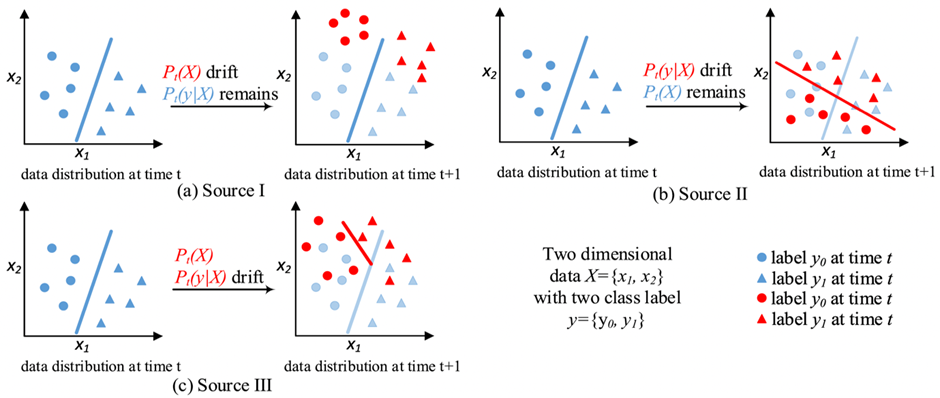
\includegraphics[width=.9\textwidth]{2_Background/figures/concept_drift_sources.png}
    \caption{Concept .}
    \caption{Concept Drift Types.}
    \label{fig:concept-drift-sources}
\end{figure}

